%
% ---------------------------------------------------------------
% Copyright (C) 2012-2018 Gang Li
% ---------------------------------------------------------------
%
% This work is the default powerdot-tuliplab style test file and may be
% distributed and/or modified under the conditions of the LaTeX Project Public
% License, either version 1.3 of this license or (at your option) any later
% version. The latest version of this license is in
% http://www.latex-project.org/lppl.txt and version 1.3 or later is part of all
% distributions of LaTeX version 2003/12/01 or later.
%
% This work has the LPPL maintenance status "maintained".
%
% This Current Maintainer of this work is Gang Li.
%
%

\documentclass[
 size=14pt,
 paper=smartboard,  %a4paper, smartboard, screen
 mode=present, 		%present, handout, print
 display=slides, 	% slidesnotes, notes, slides
 style=tuliplab,  	% TULIP Lab style
 pauseslide,
 fleqn,leqno]{powerdot}


\usepackage{cancel}
\usepackage{caption}
\usepackage{stackengine}
\usepackage{smartdiagram}
\usepackage{attrib}
\usepackage{amssymb}
\usepackage{amsmath} 
\usepackage{amsthm} 
\usepackage{mathtools}
\usepackage{rotating}
\usepackage{graphicx}
\usepackage{boxedminipage}
\usepackage{rotate}
\usepackage{calc}
\usepackage[absolute]{textpos}
\usepackage{psfrag,overpic}
\usepackage{fouriernc}
\usepackage{pstricks,pst-3d,pst-grad,pstricks-add,pst-text,pst-node,pst-tree}
\usepackage{moreverb,epsfig,subfigure}
\usepackage{color}
\usepackage{booktabs}
\usepackage{etex}
\usepackage{breqn}
\usepackage{multirow}
\usepackage{natbib}
\usepackage{bibentry}
\usepackage{gitinfo2}
\usepackage{siunitx}
\usepackage{nicefrac}
%\usepackage{geometry}
%\geometry{verbose,letterpaper}
\usepackage{media9}
\usepackage{animate}
%\usepackage{movie15}
\usepackage{auto-pst-pdf}

\usepackage{breakurl}
\usepackage{fontawesome}
\usepackage{xcolor}
\usepackage{multicol}



\usepackage{verbatim}
\usepackage[utf8]{inputenc}
\usepackage{dtk-logos}
\usepackage{tikz}
\usepackage{adigraph}
%\usepackage{tkz-graph}
\usepackage{hyperref}
%\usepackage{ulem}
\usepackage{pgfplots}
\usepackage{verbatim}
\usepackage{fontawesome}


\usepackage{todonotes}
% \usepackage{pst-rel-points}
\usepackage{animate}
\usepackage{fontawesome}

\usepackage{listings}
\lstset{frameround=fttt,
frame=trBL,
stringstyle=\ttfamily,
backgroundcolor=\color{yellow!20},
basicstyle=\footnotesize\ttfamily}
\lstnewenvironment{code}{
\lstset{frame=single,escapeinside=`',
backgroundcolor=\color{yellow!20},
basicstyle=\footnotesize\ttfamily}
}{}


\usepackage{hyperref}
\hypersetup{ % TODO: PDF meta Data
  pdftitle={Presentation Title},
  pdfauthor={Gang Li},
  pdfpagemode={FullScreen},
  pdfborder={0 0 0}
}


% \usepackage{auto-pst-pdf}
% package to show source code

\definecolor{LightGray}{rgb}{0.9,0.9,0.9}
\newlength{\pixel}\setlength\pixel{0.000714285714\slidewidth}
\setlength{\TPHorizModule}{\slidewidth}
\setlength{\TPVertModule}{\slideheight}
\newcommand\highlight[1]{\fbox{#1}}
\newcommand\icite[1]{{\footnotesize [#1]}}

\newcommand\twotonebox[2]{\fcolorbox{pdcolor2}{pdcolor2}
{#1\vphantom{#2}}\fcolorbox{pdcolor2}{white}{#2\vphantom{#1}}}
\newcommand\twotoneboxo[2]{\fcolorbox{pdcolor2}{pdcolor2}
{#1}\fcolorbox{pdcolor2}{white}{#2}}
\newcommand\vpspace[1]{\vphantom{\vspace{#1}}}
\newcommand\hpspace[1]{\hphantom{\hspace{#1}}}
\newcommand\COMMENT[1]{}

\newcommand\placepos[3]{\hbox to\z@{\kern#1
        \raisebox{-#2}[\z@][\z@]{#3}\hss}\ignorespaces}

\renewcommand{\baselinestretch}{1.2}


\newcommand{\draftnote}[3]{
	\todo[author=#2,color=#1!30,size=\footnotesize]{\textsf{#3}}	}
% TODO: add yourself here:
%
\newcommand{\gangli}[1]{\draftnote{blue}{GLi:}{#1}}
\newcommand{\shaoni}[1]{\draftnote{green}{sn:}{#1}}
\newcommand{\gliMarker}
	{\todo[author=GLi,size=\tiny,inline,color=blue!40]
	{Gang Li has worked up to here.}}
\newcommand{\snMarker}
	{\todo[author=Sn,size=\tiny,inline,color=green!40]
	{Shaoni has worked up to here.}}

%%%%%%%%%%%%%%%%%%%%%%%%%%%%%%%%%%%%%%%%%%%%%%%%%%%%%%%%%%%%%%%%%%%%%%%%
% title
% TODO: Customize to your Own Title, Name, Address
%
\title{Box Office Forecast}
\author{
Zhangtao Xue 
\\
\\Xi'an Shiyou University
%\\Deakin University
\\Chinese Academy of Sciences
%\\ \today
}
%\date{\gitCommitterDate}


% Customize the setting of slides
\pdsetup{
% TODO: Customize the left footer, and right footer
rf=\href{http://www.tulip.org.au}{
Last Changed by: \textsc{\gitCommitterName}\ \gitVtagn-\gitAbbrevHash\ (\gitAuthorDate)
},
cf={Box Office Forecast},
}


\begin{document}

\maketitle

%\begin{slide}{Overview}
%\tableofcontents[content=sections]
%\end{slide}


%%==========================================================================================
%%
\begin{slide}[toc=,bm=]{Overview}
\tableofcontents[content=currentsection,type=1]
\end{slide}
%%
%%==========================================================================================


\section{Project Overview}


%%==========================================================================================
%%
\begin{slide}{Project Introducing}
\begin{center}
\twotonebox{\rotatebox{95}{Defn}}{\parbox{.89\textwidth}
{
\begin{itemize}
\item introduce
\\With the development of the film industry, 
a variety of film and television companies
 need to predict the cost and income of shooting a 
film and television to reduce the amount of money
 spent. This software is designed to predict the
  movie revenue, etc.
~\\
\end{itemize}
}}

\end{center}
\bigskip
\begin{center}
\begin{tabular}{c| c c c c }
\toprule
\midrule

\bottomrule
\end{tabular}
\end{center}
\bigskip

%%==========================================================================================
\begin{note}
First, I will introduce the problem definition.
In the real life,
a teacher may be interested in the characteristics that
make one student obvious different from others.
Or,
NBA sports coaches would prefer to
know the advantages and disadvantages of one player.
Here, the player can be regarded as a query object.

For example, team A has five players,
each player has four features.
The NBA sports coaches may want to know the features of
player $1$ that are different from others.

The above example can be seen as outlying aspects mining.
The main purpose of outlying aspects mining is to identify
the outstanding features of the query object.
\end{note}
%%==========================================================================================

\end{slide}
%%
%%==========================================================================================


%%
%%==========================================================================================


\section{Method Adopted}


%%==========================================================================================
%%
\begin{slide}{BP Neural Network Prediction Model}
%Related Work - Outlying Aspects Mining
Back propagation network (BP network) is also known as back-propagation neural network. 
Through the training of sample data, the weights and thresholds of the network are constantly modified, 
so that the error function decreases along the negative gradient direction and approaches the expected output.  
It is a widely used neural network model, which is mostly used in function approximation, 
model recognition and classification, data compression and time series prediction. Click to open the link (example of BP neural network prediction)






%%==========================================================================================
\begin{note}
Let me introduce two existing methods:
Feature selection and score-and-search.

For feature selection,
the query point can be regarded as positive class and
the rest of the data can be regarded as negative class,
selected the features that best distinguish the two classes.

The advantages of this method are easy to operate,
and it's able to resolve dimensionality bias.
However, it has some drawbacks.
Firstly,
positive and negative classes are Not balanced,
secondly,
it can't quantify the outlying degree correctly.
Most importantly,
it doesn't identify group outlying aspects.
\end{note}
%%==========================================================================================

\end{slide}
%%
%%==========================================================================================

%%
%%==========================================================================================

\section{Data}

%%==========================================================================================
%%

%%
%%===========================================================================================



%%
%%=============================================================================================
\begin{slide}[toc=,bm=]{ Data Related Operations}
\begin{itemize}
\item Data Collection
\\The data set directly obtained in kaggle    
\item 
Data Processing
\\The processing of useless data

\end{itemize}
\begin{figure}[htbp]
  \centering
  \begin{minipage}[t]{0.48\textwidth}
    \centering
    \includegraphics[width=0.9\textwidth]{logos/21.eps}
    \vspace{0.4em}
    \caption{Download dataset display from kaggle}
  \end{minipage}
  \begin{minipage}[t]{0.48\textwidth}
    \centering
    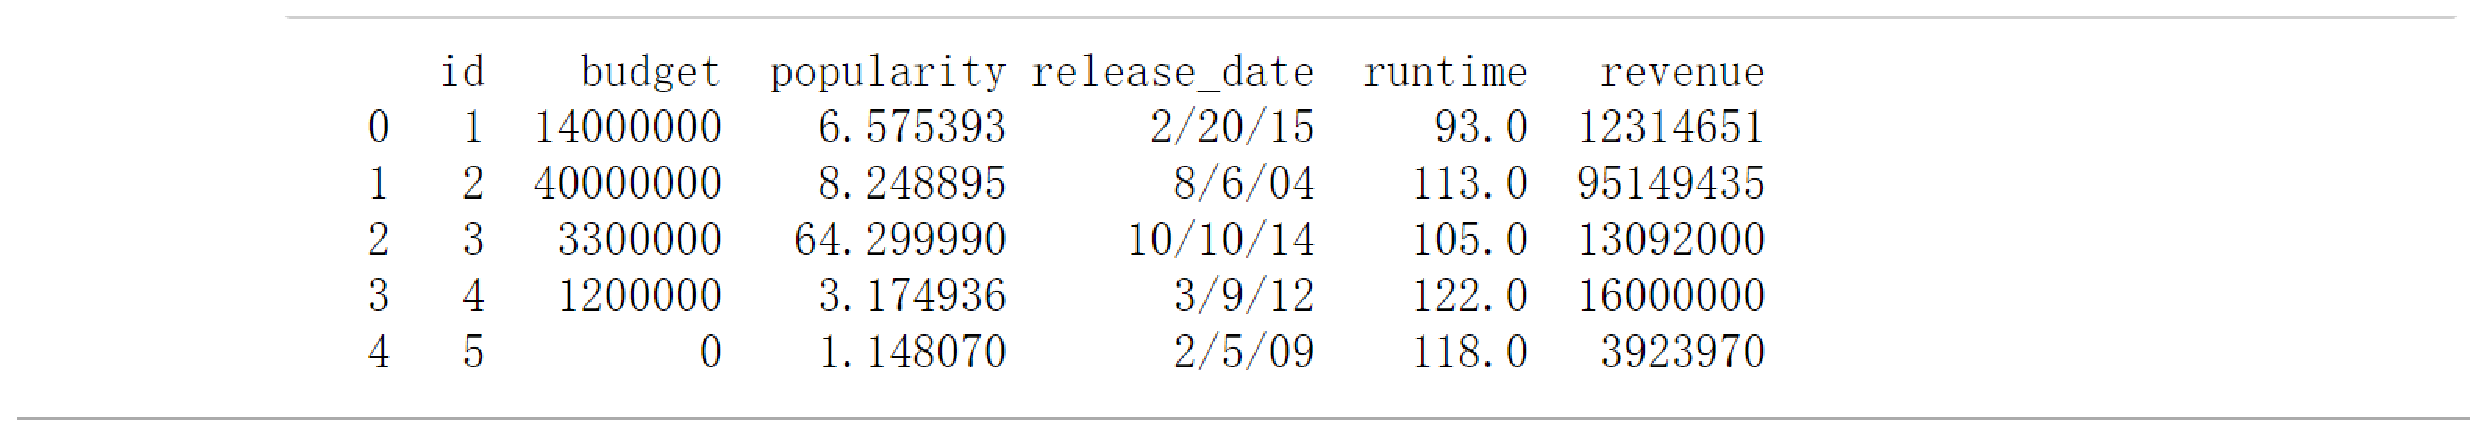
\includegraphics[width=0.9\textwidth]{logos/24.eps}
    \vspace{0.4em}
    \caption{Remove the data that has little influence on the weight}
  \end{minipage}
\end{figure}
%%==========================================================================================
\begin{note}
In conclusion,
we firstly formalized the problem of
group outlying aspects mining,

Then proposed a novel method GOAM algorithm to address the problem of
group outlying aspects mining,
and the proposed method use pruning to reduce time complexity
while identifying the suitable set of outlying features for the interested group.

Thank you and any question?
\end{note}
%%==========================================================================================

\end{slide}


\begin{slide}[toc=,bm=]{ Data Related Operations}
  \begin{itemize}
  \item The relationship between time and business income
  
  \item Relationship between runtime and business income
  

  
  \end{itemize}
  \begin{figure}[htbp]
    \centering
    \begin{minipage}[t]{0.48\textwidth}
      \centering
      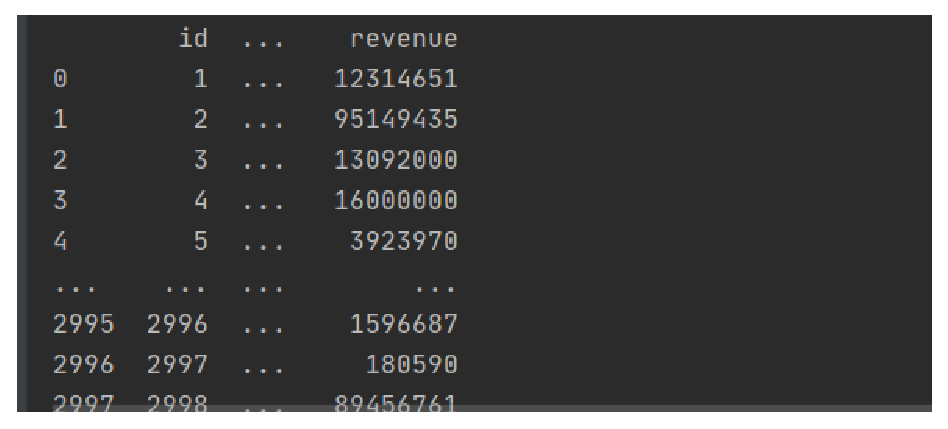
\includegraphics[width=0.9\textwidth]{logos/4.eps}
      \vspace{0.4em}
      \caption{time}
    \end{minipage}
    \begin{minipage}[t]{0.48\textwidth}
      \centering
      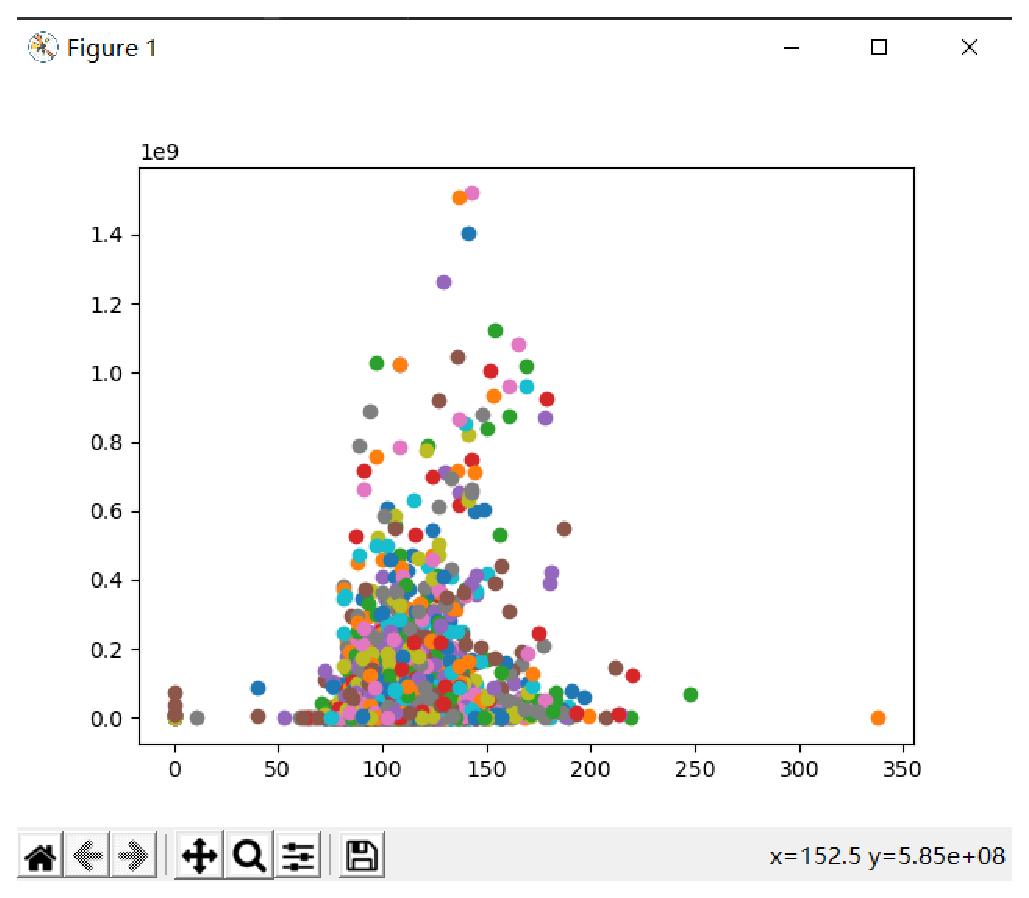
\includegraphics[width=0.9\textwidth]{logos/22.eps}
      \vspace{0.4em}
      \caption{runtime}
    \end{minipage}
  \end{figure}
  %%==========================================================================================
  \begin{note}
  In conclusion,
  we firstly formalized the problem of
  group outlying aspects mining,
  
  Then proposed a novel method GOAM algorithm to address the problem of
  group outlying aspects mining,
  and the proposed method use pruning to reduce time complexity
  while identifying the suitable set of outlying features for the interested group.
  
  Thank you and any question?
  \end{note}
  %%==========================================================================================
  
  \end{slide}
%%
%%==========================================================================================
\begin{slide}[toc=,bm=]{ Data Related Operations}
  \begin{itemize}
  \item The relationship between the prophase investment and business income of films
  
  \item The relationship between popularity and business income
 

  
  \end{itemize}
  \begin{figure}[htbp]
    \centering
    \begin{minipage}[t]{0.48\textwidth}
      \centering
      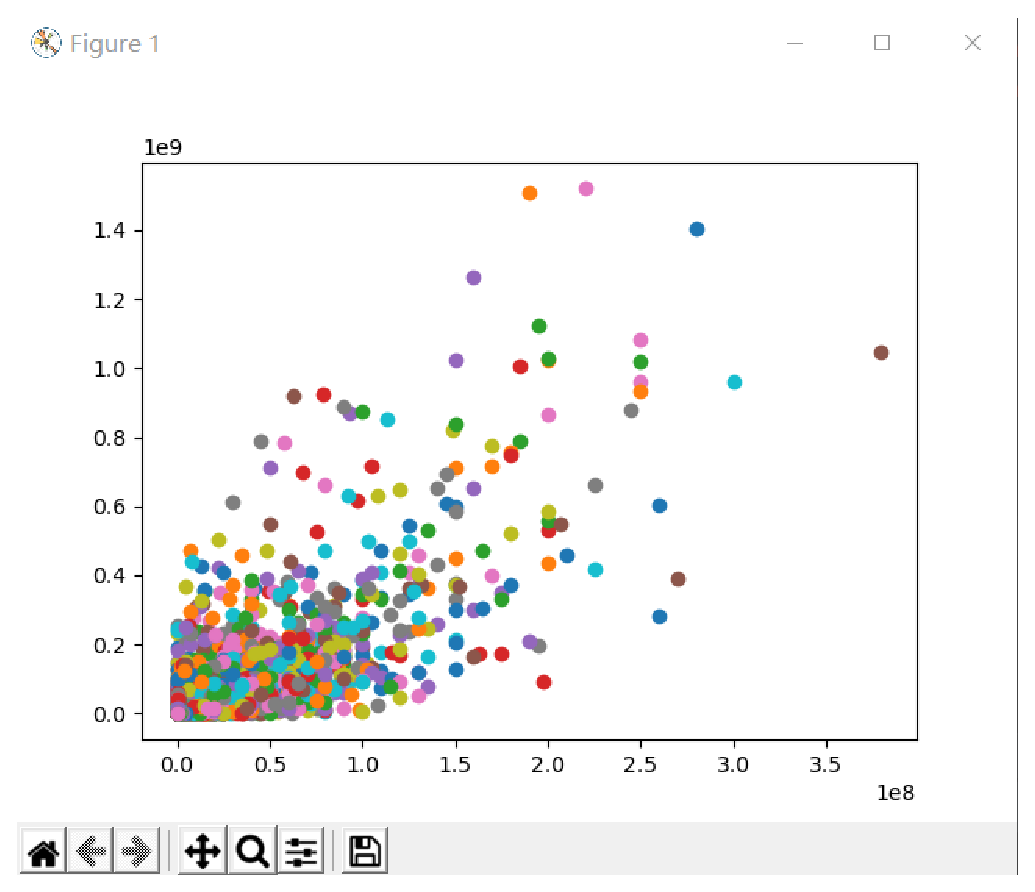
\includegraphics[width=0.9\textwidth]{logos/25.eps}
      \vspace{0.4em}
      \caption{investment}
    \end{minipage}
    \begin{minipage}[t]{0.48\textwidth}
      \centering
      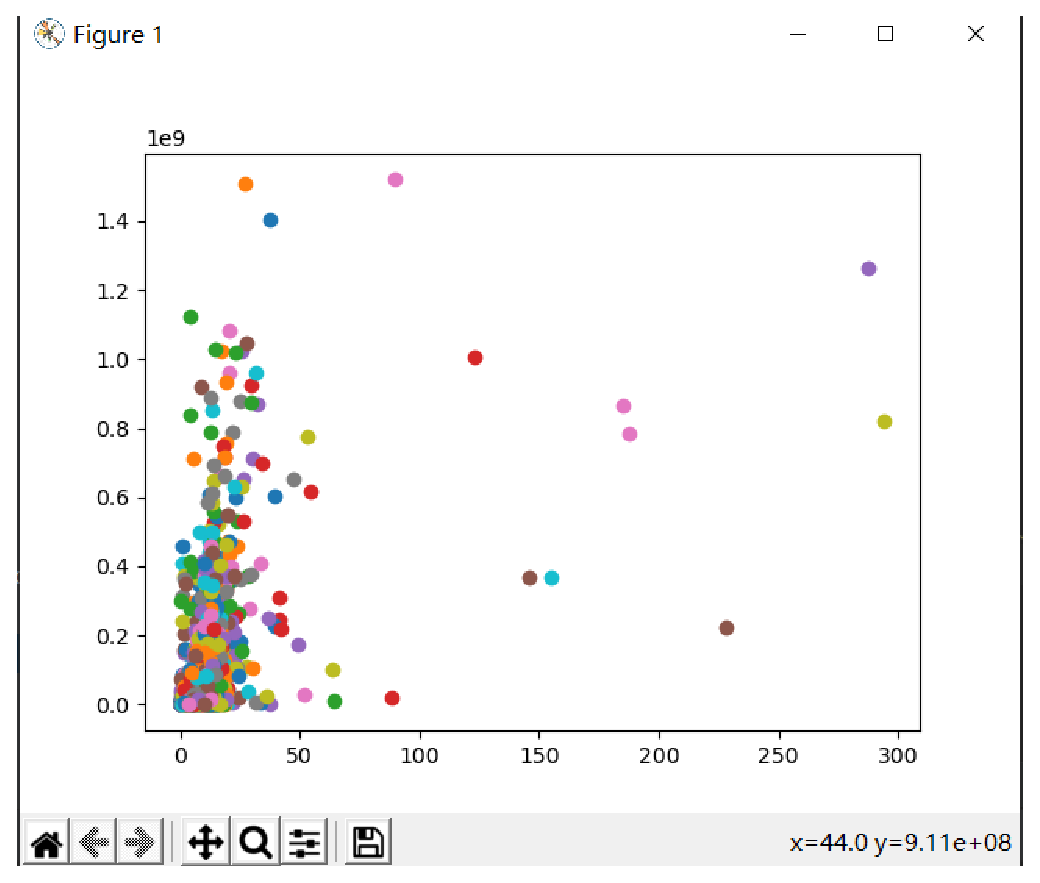
\includegraphics[width=0.9\textwidth]{logos/26.eps}
      \vspace{0.4em}
      \caption{popularity}
    \end{minipage}
  \end{figure}
  %%==========================================================================================
  \begin{note}
  In conclusion,
  we firstly formalized the problem of
  group outlying aspects mining,
  
  Then proposed a novel method GOAM algorithm to address the problem of
  group outlying aspects mining,
  and the proposed method use pruning to reduce time complexity
  while identifying the suitable set of outlying features for the interested group.
  
  Thank you and any question?
  \end{note}
  %%==========================================================================================
  
  \end{slide}
  

%%
%%===========================================================================================

\section{Model Training And Testing} 

%%===========================================================================================
%%


%%
%%==============================================================================================
\begin{slide}{Training And Testing}


\begin{itemize}
  \item Cost function selection and neural network structure selection
\item  Display of test data
\end{itemize}

\begin{figure}[htbp]
  \centering
  \begin{minipage}[t]{0.38\textwidth}
    \centering
    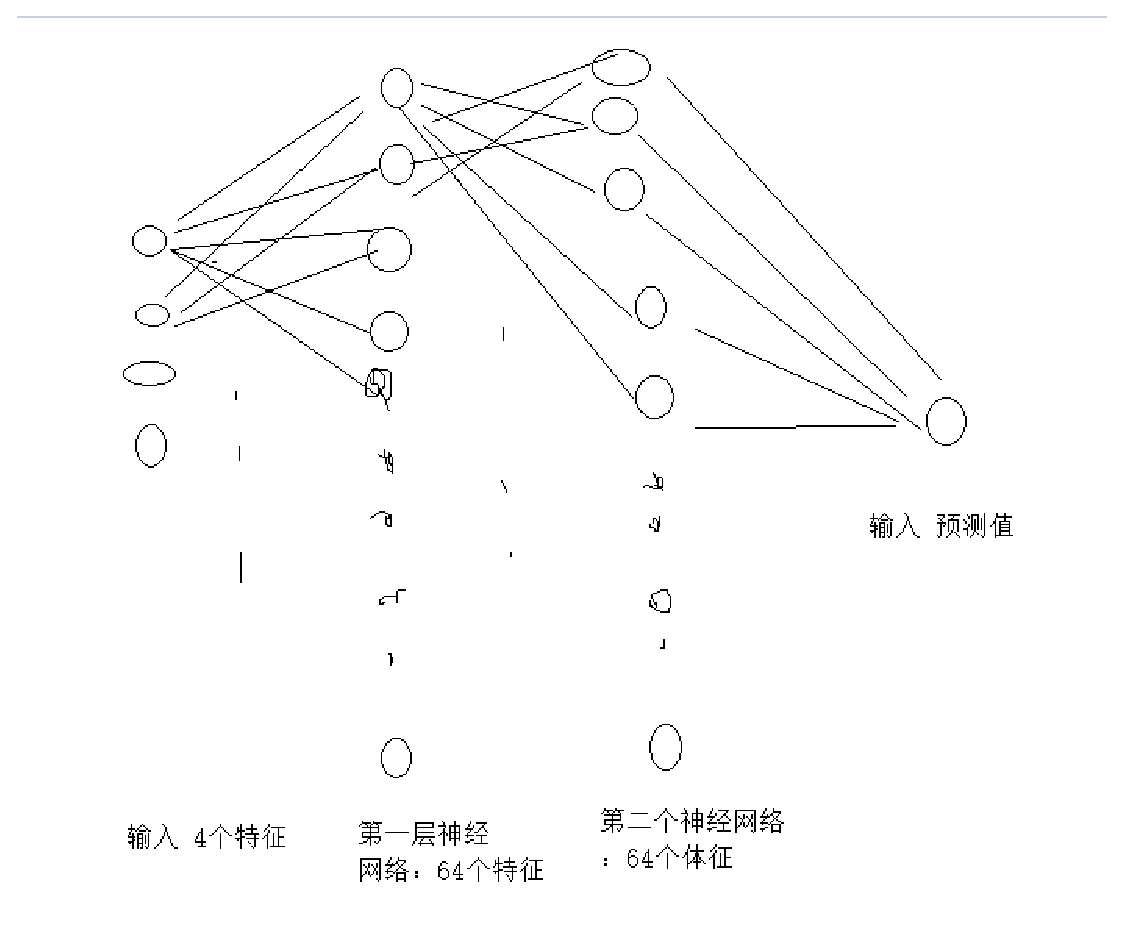
\includegraphics[width=0.7\textwidth]{logos/7.eps}
    \vspace{-1.0em}
    \caption{precdtion}
  \end{minipage}
  \begin{minipage}[t]{0.38\textwidth}
    \centering
    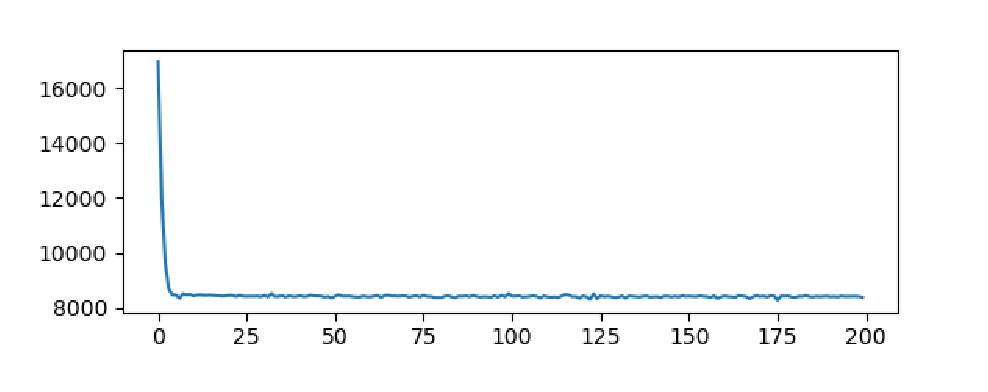
\includegraphics[width=0.7\textwidth]{logos/1 (1).eps}
    \vspace{-1.0em}
    \caption{loss  upate }
  \end{minipage}
  \begin{minipage}[t]{0.38\textwidth}
    \centering
    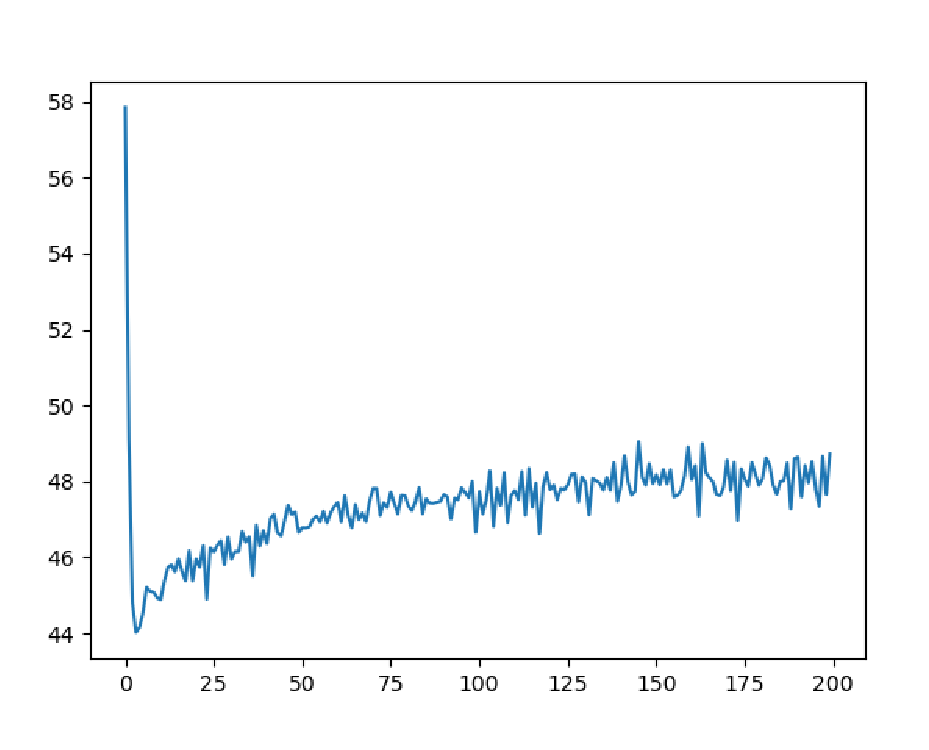
\includegraphics[width=0.7\textwidth]{logos/1 (2).eps}
    \vspace{-1.0em}
    \caption{mean_absolute_error}
  \end{minipage}
  \begin{minipage}[t]{0.38\textwidth}
    \centering
    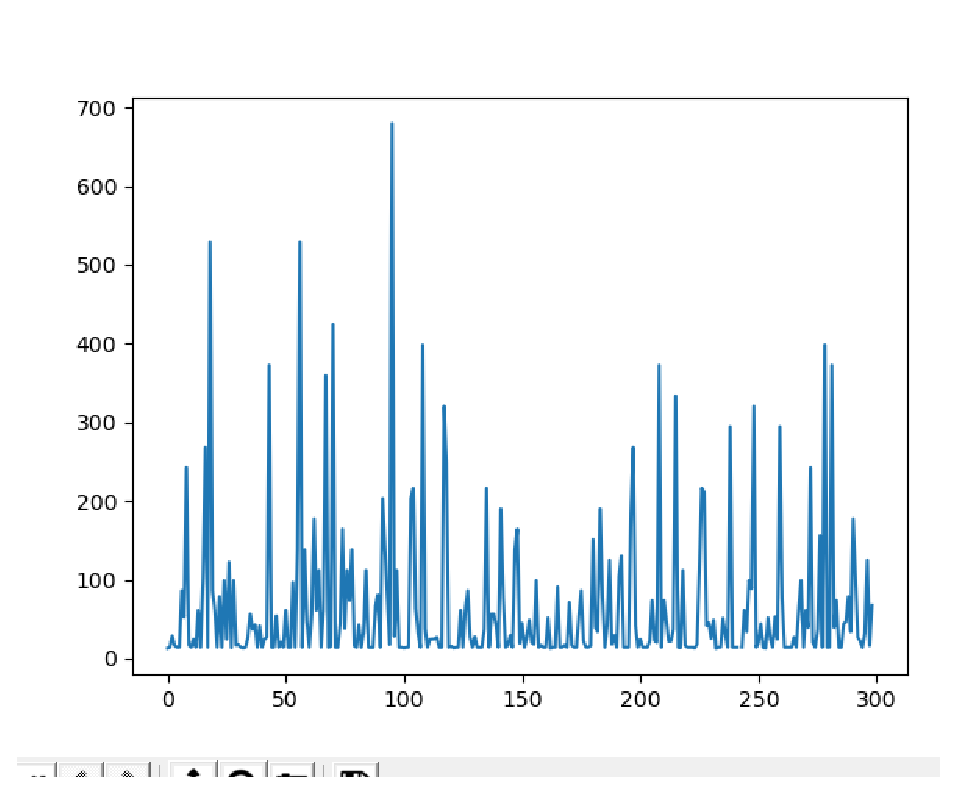
\includegraphics[width=0.7\textwidth]{logos/1 (3).eps}
    \vspace{-1.0em}
    \caption{precdtion}
  \end{minipage}
  
\end{figure}
\end{slide}

%%
%%===============================================================================================




%%==========================================================================================
%%


\section{conclusion}

\begin{slide}{conclusion}
  %Related Work - Outlying Aspects Mining
  Summary: problem: in the actual test process: in the process of numerical calculation, the large value results in the program running error.a deeper understanding of logical regression

  
  
  
  %%==========================================================================================
  \begin{note}
  Let me introduce two existing methods:
  Feature selection and score-and-search.
  
  For feature selection,
  the query point can be regarded as positive class and
  the rest of the data can be regarded as negative class,
  selected the features that best distinguish the two classes.
  
  The advantages of this method are easy to operate,
  and it's able to resolve dimensionality bias.
  However, it has some drawbacks.
  Firstly,
  positive and negative classes are Not balanced,
  secondly,
  it can't quantify the outlying degree correctly.
  Most importantly,
  it doesn't identify group outlying aspects.
  \end{note}
  %%==========================================================================================
  
  \end{slide}
% TODO: Contact Page
\end{document}

\endinput
